%!TEX root = ../dokumentation.tex
\chapter{Implementation}

The implementation of ARIMA needs two separate scripts: One for predictions/forecasting and one for training a suitable model.
Naturally the training script is going to use the prediction script in some way to test the current model and improve it.

Both scripts need to do three things: 
First, loading the time series and parameters p, d, q, P, D, Q, and s. Then differencing the time series according to d and D. And finally they both have to construct the auxiliary matrix $Z$. This matrix is needed to do different calculations within both scripts. The idea behind it, is to provide all the $X_{t-h}$ for any $h \in [1, max(p, q, Ps, Qs, p + Ps, q + Qs]$ for each $\hat{X}_t$ to be computed.
This means that there is p columns for \acs{AR}$(p)$, q columns for \acs{MA}$(q)$, P columns for \acs{SAR}$(P)$, Q columns for \acs{SMA}$(Q)$ and when combining non seasonal and seasonal models there is also additional $p \cdot P$ and $q \cdot Q$ columns. Each one of those columns corresponds to one of the $X_{t-h}$ terms found in equation for \eqref{eq:multiplicative_SARIMA}. So essentially Z is constructed in a way that the n-th row of Z contains all the time series values needed to predict $X_n$.

\begin{figure}[ht]
	\centering
	\scalebox{1}{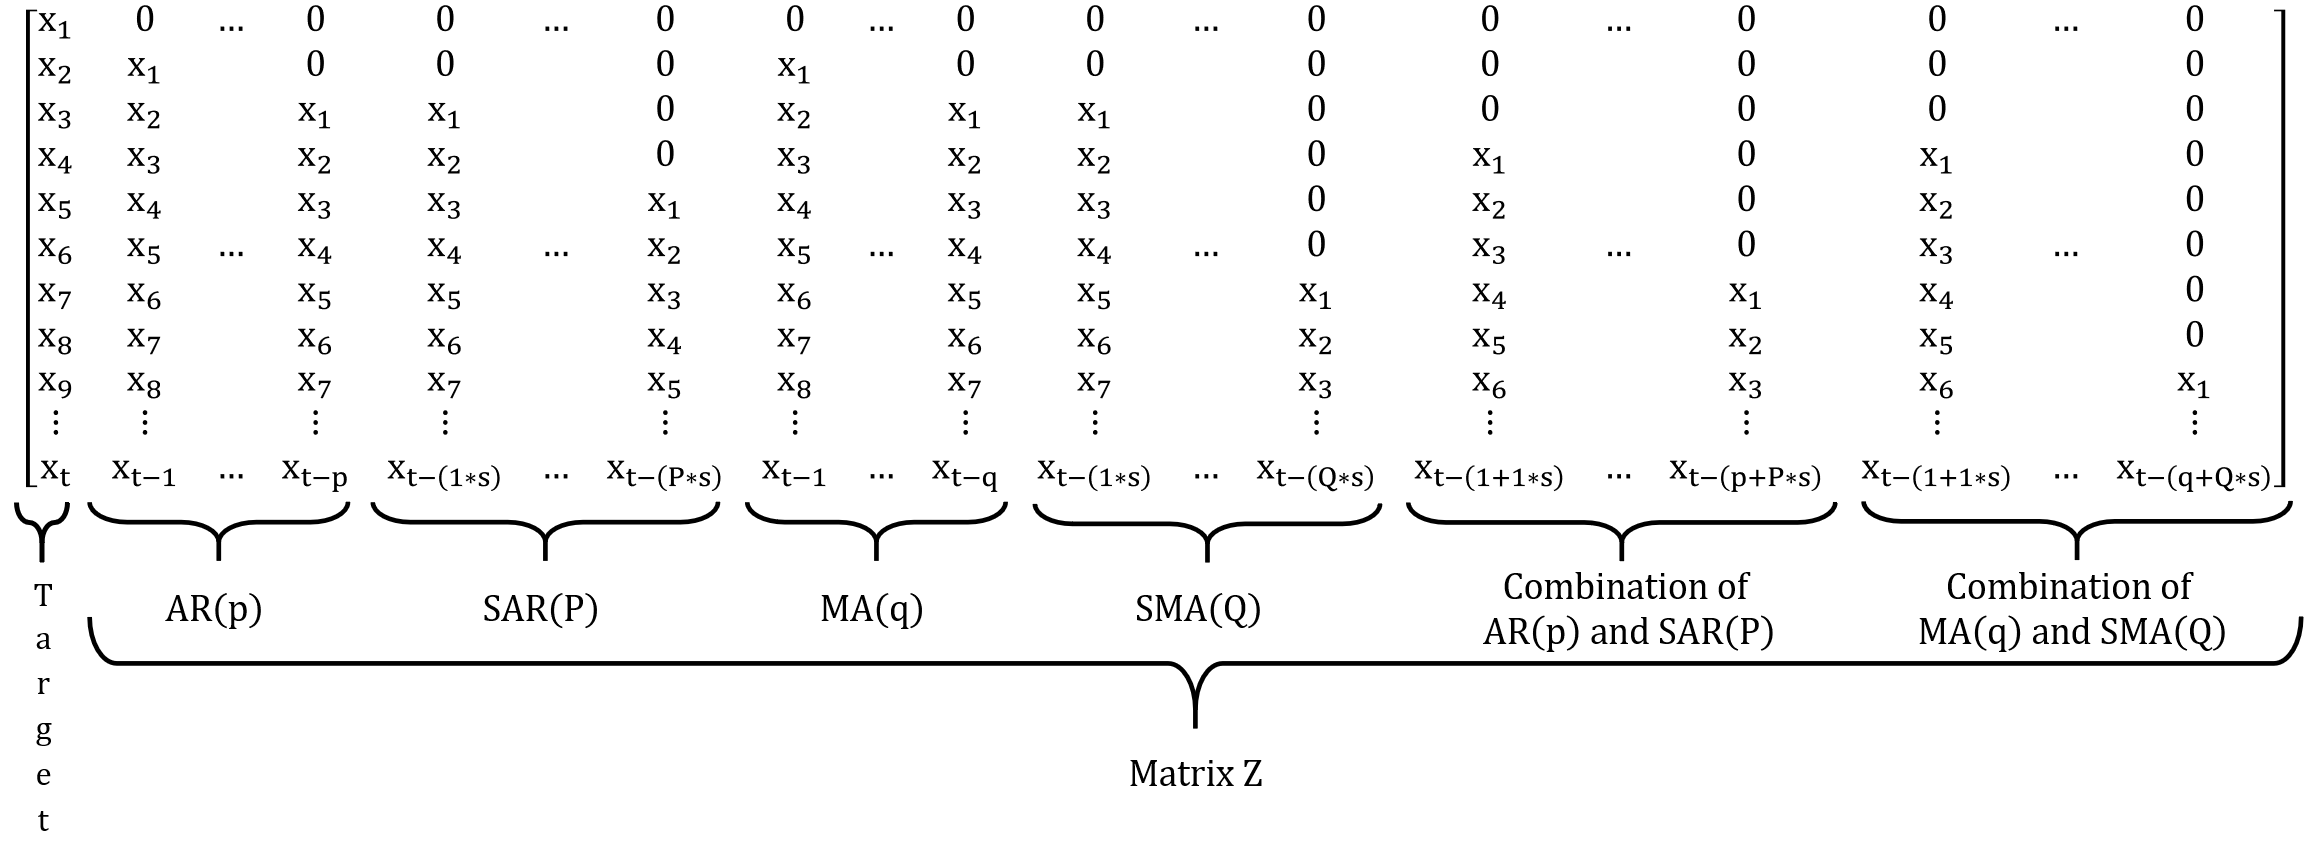
\includegraphics[width=1\textwidth]{images/Zmatrix.png}}
    \caption{Schema of auxiliary matrix Z}
\end{figure}

The following function is designed to built such a matrix:
\begin{lstlisting}[caption=Prediction of \acs{AR}$(p)$ or  \acs{SAR}$(P)$ ,captionpos=b]
constructPredictorMatrix = function (Matrix[Double] X, Integer p, Integer P, Integer q, Integer Q, Integer s)return( Matrix[Double] Z){
	Z = matrix(0, nrow(X), p+P+Q+q+p*P+q*Q)

	# fills Z with values used for non seasonal AR prediction
	for	(i in seq(1, p, 1)){
		Z = addShiftedMatrix(Z, X, i, i)
	}

	#prediction values for seasonal AR 
	for(i in seq(1, P, 1)){
		Z = addShiftedMatrix(Z, X, (i * s), p + i)
	}

	#prediction values for combined models of non-seasonal and seasonal AR
	Z = addValuesForCombinedModel (Z, X, p, P, s, p + P)

	#prediction values for non seasonal MA 
	for(i in seq(1, q, 1)){
		Z = addShiftedMatrix(Z, X, i, p + P + p*P + i)
	}

	#prediction values for seasonal MA 
	for(i in seq(1,Q, 1)){
		Z = addShiftedMatrix(Z, X, (i * s), p + P + p*P + q + i)
	}

	#prediction values for combined models of non-seasonal and seasonal MA
	Z = addValuesForCombinedModel (Z, X, q, Q, s, p + P + p*P + q + Q )
}
\end{lstlisting}

The idea behind this function is to add each column step by step. It starts with all the columns for non seasonal and seasonal \acl{AR} and proceeds to \acl{MA}.


%TODO: Maybe add example of Z matrix here

\section{Prediction Script}

The task of the prediction script is simply to calculate the t-dimensional vector $\hat{X}$ containing all the predictions $\hat{X}_t$ for each $t \in [1,T]$ with T being the number of rows of  $Z$. When using the prediction script for training purposes this is also equal to the size of the time series $X$ used for training.

In the simplest case of forecasting \acs{AR}$(p)$ or  \acs{SAR}$(P)$  the code for the \lstinline{predict()} function is quite straight forward:

\begin{lstlisting}[caption=Prediction of \acs{AR}$(p)$ or  \acs{SAR}$(P)$ ,captionpos=b]
predict = function(Matrix[Double] weights, Matrix[Double] Z) return (Matrix[Double] approximated_solution){
	approximated_solution = Z%*%weights
}
\end{lstlisting}

For predicting non seasonal and seasonal \acs{SAR} at once the combination of the purely non seasonal and purely seasonal part have to be taken into consideration. This is done by constructing another auxiliary matrix $\omega$ (referred to in the scripts as 'combined\_weights') that holds all weights for $p$ and $P$ as well as all the combinations of those weights:

\begin{lstlisting}[caption=Prediction of \acs{SAR}$(p)(P)$ ,captionpos=b]
combined_weights = weights
if (p>0 & P>0){
	combined_weights = rbind(combined_weights, matrix(weights[1:p,] %*% t(weights[p+1:p+P,]), rows=p*P, cols=1))
}
approximated_solution = Z%*%combined_weights
\end{lstlisting}

Like already discussed in the chapter \ref{arimamodel} and described in more detail with the equations \eqref{eq:MA_q} through \eqref{eq:example_MA_three_system_2}, calculating $\hat{X}$ for \acs{MA}(p) requires to construct a third matrix R to be used to describe the system of linear equations that needs to be solved with:
\[A = I + R\]

\begin{lstlisting}[caption=Prediction of \acs{MA}$(q)$ ,captionpos=b]
b = Z%*%weights
R = matrix(0, nrow(Z), nrow(Z))
for(i in seq(1, q, 1)){
	d_ns = matrix(as.scalar(weights[P+p+i,1]), nrow(R)-i, 1)
	R[1+i:nrow(R),1:ncol(R)-i] = R[1+i:nrow(R),1:ncol(R)-i] + diag(d_ns)
}
approximated_solution = numerical_solvers::jacobi (A=A, b=b)
\end{lstlisting}

The equivalent for-loop can be implemented for \acs{SMA} as well. With the only difference that instead of the term $i$ the term $i\cdot s$ is to be used.

To solve the system of linear equations the \textit{Jacobi} solver had to be implemented in the way it was described in chapter \ref{jacobi}:
\begin{lstlisting}[caption=Prediction of \acs{MA}$(q)$ ,captionpos=b]
jacobi = function (Matrix[Double] R, Matrix[Double] b, Double tolerance = 0.01, Integer max_iterations = 1000)  return (Matrix[Double] x){
	x = matrix(0, nrow(R), 1)
  	k = 0
	diff = tolerance+1
	while(k < max_iterations & diff > tolerance){
		x_k = b - R%*%x
		diff = sum((x_k-x)^2)
		x = x_k
		k += 1
	}
}
\end{lstlisting}

\section{Training Script}


%Pseudo code/description arima training

%Load Time Series X_t and parameters p, d, q, P, D, Q, and s
%Difference X_tnon seasonaland seasonal
%Build auxiliary matrix Z with the series X_t  as the first column, the target values and all the previous values from X_t that can be used to predict the target value at time  
%Solve nonlinear optimization problem for ARMA(p,q)〖(P,Q)〗_s   to find best values for 〖 ϕ〗_i,〖 Φ〗_j,〖 θ〗_k,〖 Θ〗_l over a) Maximum likelihood estimation b) Nonlinear least squares method  



%arima residuals and css 
%gradient of arima
%bfgs

%building Z
	%addshiftedMatrix
    %addValuesForCombinedModel
    
%differencing

\chapter{Result}
% What was tested

\section{Correctness Test}

\section{Performance Test}


















